\documentclass{standalone}
\usepackage{unicode-math}
\usepackage{amsmath}
\usepackage{tikz}
\usepackage{fontspec}
\setmainfont{DejaVu Sans}

\usetikzlibrary{automata,arrows,positioning,calc,snakes}

\begin{document}

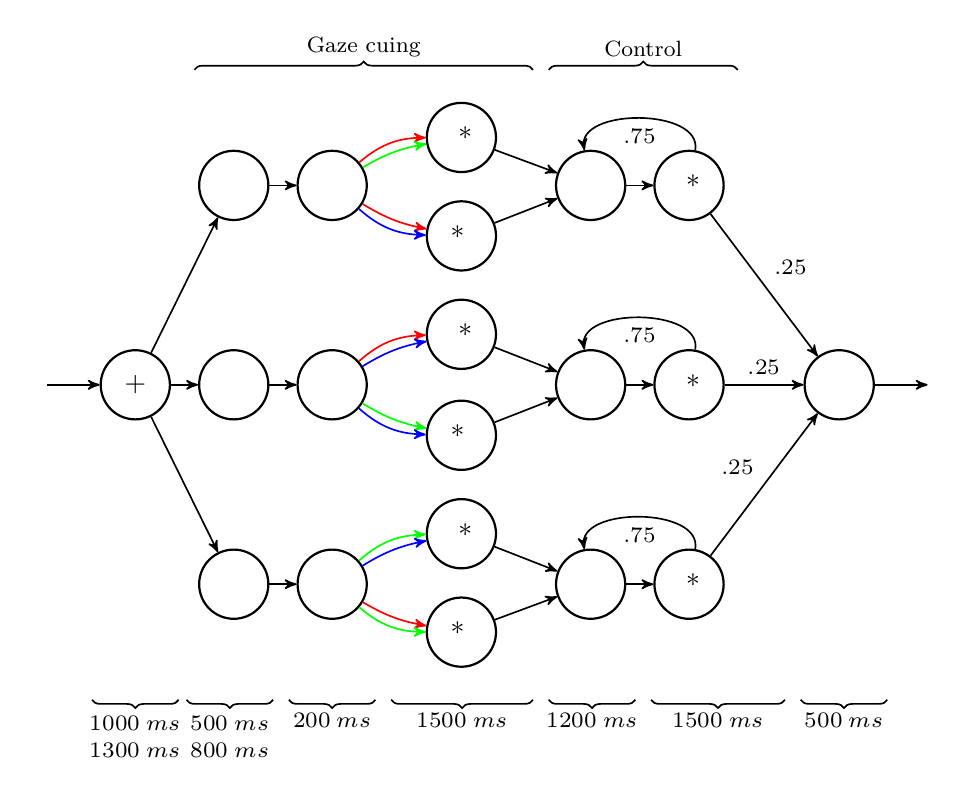
\begin{tikzpicture}[->, >=stealth', auto, semithick, node distance=1.25cm]
    \tikzstyle{every state}=[fill=white,draw=black,thick,text=black,scale=1]

    \node[state] (☺){☺};        %happy
    \node[state] (😏)[right of=☺] {😏};        % happy averted
    \node[state] (😏*)[above right=0cm and 1cm of 😏]                     {😏*}; %happy congruent
    \node[state] (*😏)[below right=0cm and 1cm of 😏]                     {*😏}; %happy incongruent
    \node[state] (☺2)[below right=0cm and 1cm of 😏*] {☺};        %happy2
    \node[state] (☺*)[right of=☺2] {☺*}; %happy null

    \node[state] (*😒)[above of=😏*]                     {*😒}; %neutral incongruent
    \node[state] (😒)[above left =0cm and 1cm of *😒]             {😒}; %neutral averted
    \node[state] (😐)[left of=😒]                             {😐}; %neutral
    \node[state] (😒*)[above of=*😒]                     {😒*}; %neutral congruent
    \node[state] (😐2)[above right =0cm and 1cm of *😒]             {😐}; %neutral
    \node[state] (😐*)[right of=😐2]                     {😐*}; %neutral null

    \node[state] (😒**)[below of=*😏]   {😒*}; %sad congruent
    \node[state] (😒averted)[below left=0cm and 1cm of 😒**] {😒};         %sad averted
    \node[state] (☹)[left of=😒averted] {☹};
    \node[state] (**😒)[below of=😒**] {*😒}; %sad incongruent
    \node[state] (☹2)[below right=0cm and 1cm of 😒**] {☹};         %sad null
    \node[state] (☹*)[right of=☹2]                     {☹*}; %sad null

    % fixation point
    \node[state] (+)[left of=☺] {+};             % fixation point
    \node (start)[left of=+] {};
    \node[state] (end)[right=1cm of ☺*] {};
    \node (endend)[right of=end] {};

    % edges
    \path(start) edge (+);
    \path(+) edge (😐);
    \path(+) edge (☹);
    \path(+) edge (☺);

    \path(😐) edge (😒);
    \path (😒) edge[bend left=20,red] (😒*);
    \path (😒) edge[bend left=10,green] (😒*);
    \path (😒) edge[bend right=10,red] (*😒);
    \path (😒) edge[bend right=20,blue] (*😒);

    \path(☺) edge (😏);
    \path(😏) edge[bend left=20,red] (😏*);
    \path(😏) edge[bend left=10,blue] (😏*);
    \path(😏) edge[bend right=10,green] (*😏);
    \path(😏) edge[bend right=20,blue] (*😏);

    \path(☹) edge (😒averted);
    \path(😒averted) edge[bend left=20,green] (😒**);
    \path(😒averted) edge[bend left=10,blue] (😒**);
    \path(😒averted) edge[bend right=10,red] (**😒);
    \path(😒averted) edge[bend right=20,green] (**😒);

    % 2nd-to-3rd column edges
    \path(😒*) edge (😐2);
    \path(*😒) edge (😐2);
    \path(😐2) edge  (😐*);
    \path(😐*) edge[bend right=100] node{\footnotesize $.75$} (😐2);
    \path(😐*) edge node{\footnotesize $.25$} (end);

    \path(😏*) edge (☺2);
    \path(*😏) edge (☺2);
    \path(☺2) edge (☺*);
    \path(☺*) edge[bend right=100] node{\footnotesize $.75$} (☺2);
    \path(☺*) edge node{\footnotesize $.25$} (end);

    \path(😒**) edge (☹2);
    \path(**😒) edge (☹2);
    \path(☹2) edge (☹*);
    \path(☹*) edge[bend right=100] node{\footnotesize $.75$} (☹2);
    \path(☹*) edge node{\footnotesize $.25$} (end);

    \path(end) edge (endend);

    % braces (timeline and contrasts)
    \draw[-,decorate,decoration={brace,amplitude=3pt,mirror}] (-1.8,-4)
        -- (-.7,-4) node[pos=0.5,anchor=north,yshift=-1]
        {\footnotesize  $\begin{array}{c} 1000\;ms \\
                                          1300\;ms \\
                        \end{array}$};
    \draw[-,decorate,decoration={brace,amplitude=3pt,mirror}] (-.6,-4)
        -- (.5,-4) node[pos=0.5,anchor=north,yshift=-1]
        {\footnotesize  $\begin{array}{c} 500\;ms \\
                                          800\;ms \\
                        \end{array}$};
    \draw[-,decorate,decoration={brace,amplitude=3pt,mirror}] (.7,-4)
        -- (1.8,-4) node[pos=0.5,anchor=north,yshift=-1]{\footnotesize  $200\;ms$};
    \draw[-,decorate,decoration={brace,amplitude=3pt,mirror}] (2,-4)
        -- (3.8,-4) node[pos=0.5,anchor=north,yshift=-1]{\footnotesize  $1500\;ms$};
    \draw[-,decorate,decoration={brace,amplitude=3pt,mirror}] (4,-4)
        -- (5.1,-4) node[pos=0.5,anchor=north,yshift=-1]{\footnotesize  $1200\;ms$};
    \draw[-,decorate,decoration={brace,amplitude=3pt,mirror}] (5.3,-4)
        -- (7,-4) node[pos=0.5,anchor=north,yshift=-1]{\footnotesize  $1500\;ms$};
    \draw[-,decorate,decoration={brace,amplitude=3pt,mirror}] (7.2,-4)
       -- (8.3,-4) node[pos=0.5,anchor=north,yshift=-1]{\footnotesize  $500\;ms$};

    \draw[-,decorate,decoration={brace,amplitude=3pt}] (-.5,4)
        -- (3.8,4) node[pos=0.5,yshift=1]{\footnotesize  Gaze cuing};
    \draw[-,decorate,decoration={brace,amplitude=3pt}] (4,4)
        -- (6.4,4) node[pos=0.5,yshift=1]{\footnotesize  Control};

  \end{tikzpicture}
\end{document}
